\documentclass[a4paper]{article}
\usepackage[pdftex]{graphicx}
\usepackage{float}
\usepackage{hyperref}
\usepackage{listings}
\usepackage{amssymb}
\floatstyle{ruled}
\newfloat{listing}{hbtH}{lop}
\floatname{listing}{Listing}
\renewcommand{\topfraction}{0.85}   % This sets the percentage for how much floats get from the ‘top’ of the text of a page
\renewcommand{\textfraction}{0}   % This sets a similar percentage for how much of a page needs to be text before no more floats can be placed on that page
\renewcommand{\floatpagefraction}{0.80} % This sets how much of the page must be taken by a float before that page can be ‘all’ floats

\newcommand{\subtypeeq}{\sqsubseteq}
\newcommand{\subtype}{\sqsubset}

\author{Etienne Kneuss\\
\texttt{etienne.kneuss@epfl.ch}
}
\title{Insane: Interprocedural Static Analysis Engine for Scala}
%\bibiographystyle{unsrt}
\begin{document}
\maketitle
\begin{abstract}
  This report presents the work that was done during the winter semester
  2011-2012. It describes the various improvements and refinements that
  were applied to the original analysis.
\end{abstract}
\section{Introduction}
Insane is a pointer and effect analysis for Scala applications. It is meant to
compute and combine modular effects, with various degrees of precision. It was
specifically designed to address higher-order functions -- or equivalently
precise handling of dynamic dispatch. Insane is composed of a combination of
two analyses:

\begin{enumerate}
    \item a precise, intra-procedural but flow-sensitive \textbf{type analysis}
    \item a modular, inter-procedural pointer and \textbf{effect analysis}
\end{enumerate}

\section{Type Analysis}
\subsection{Overview}
Object oriented languages such as Scala implement \emph{dynamic dispatch}: the
target of a method call is only determined at runtime, based on the actual
runtime type of the receiver. This feature is essential in object oriented
languages as it allows subtype polymorphism. Obtaining precise information on
the possible runtime types of those receivers will allow us to construct a
precise call-graph.

Type analysis is responsible to compute an over approximation of the set of
actual concrete types a variable could hold at runtime. Given a variable
\verb=v : T=, we know that its static type \verb=T= already provides a valid
bound on the set of possible concrete types, but this information is not
precise enough in practice. This analysis is designed to improve this static
bound by tracking how allocated objects flow in a procedure and derive more
precise type constraints. We use abstract interpretation using sets of type
constraints as abstract values.

\subsection{Handling Casts Precisely}
The only sensible improvement that was applied to this analysis is the precise
handling of casts. Previously, casting an object would generate a type
constraint corresponding to the type used in the cast. This follows the type
rules of Scala. While valid, it is not precise enough. We instead
re-implemented it using type intersection. Type intersection between two sets
of type constraints $C_1$ and $C_2$ is defined by:

\begin{eqnarray*}
        C_1 \cap C_2 := \bigcup_{(c_1,c_2) ~ \in ~ Cs_1 \times Cs_2} \{ T ~|~ T \models c_1 \land T \models c_2  \}
\end{eqnarray*}

Type intersection allows us to model precisely the possible types resulting
from a type cast. We illustrate this with an example:


\begin{lstlisting}
    trait A
    trait B
    class T1 extends A with B
    class T2 extends B

    val a: A = ...

     ...

    if (...) {
        val b: B = a.asInstanceOf[B]

         ...

    }
\end{lstlisting}


While the static type of \verb=b= is \verb=B=, type intersection will give us a
more detailled description of objects stored in \verb=b=. In fact, only objects that
are both of type \verb=A= and \verb=B= will be valid candidates. In the example,
the result of type intersection will give us the constraint $\_ \subtypeeq T1$,
which allows only $T1$ in our case. The constraint obtained from the static
type, $\_ \subtypeeq B$, would allow for $T2$ as well which is not possible in
our case.

\subsection{Evaluation}
It is not obvious whether this simple analysis will give interesting results.
The main purpose being to compute the call-graph, we will focus on the
improvements obtained for method calls. That is, for each method call, we
compare the number of targets that we obtain with and without refined type
constraints. We use the official Scala library as benchmark. It is our belief
that the library is representative of typical Scala applications for the
purpose of this analysis.

The Scala library contains 122'980 method calls at the compiler phase we
operate. However, only 18'611 of them have a non-unique \emph{static} target.
We represent the improvements provided by our analysis using the scatter plot
in Figure~\ref{fig:scatter}. We can see that the improvements are often
important. Also, we notice that this analysis is at least as precise as the
static type is: it is only improving the set of targets. In overall we obtain
1'278'384 edges in our refined call graph, instead of 3'554'422 without the
analysis, which represents a 64\% reduction.

\begin{figure}[h]
    \begin{center}
    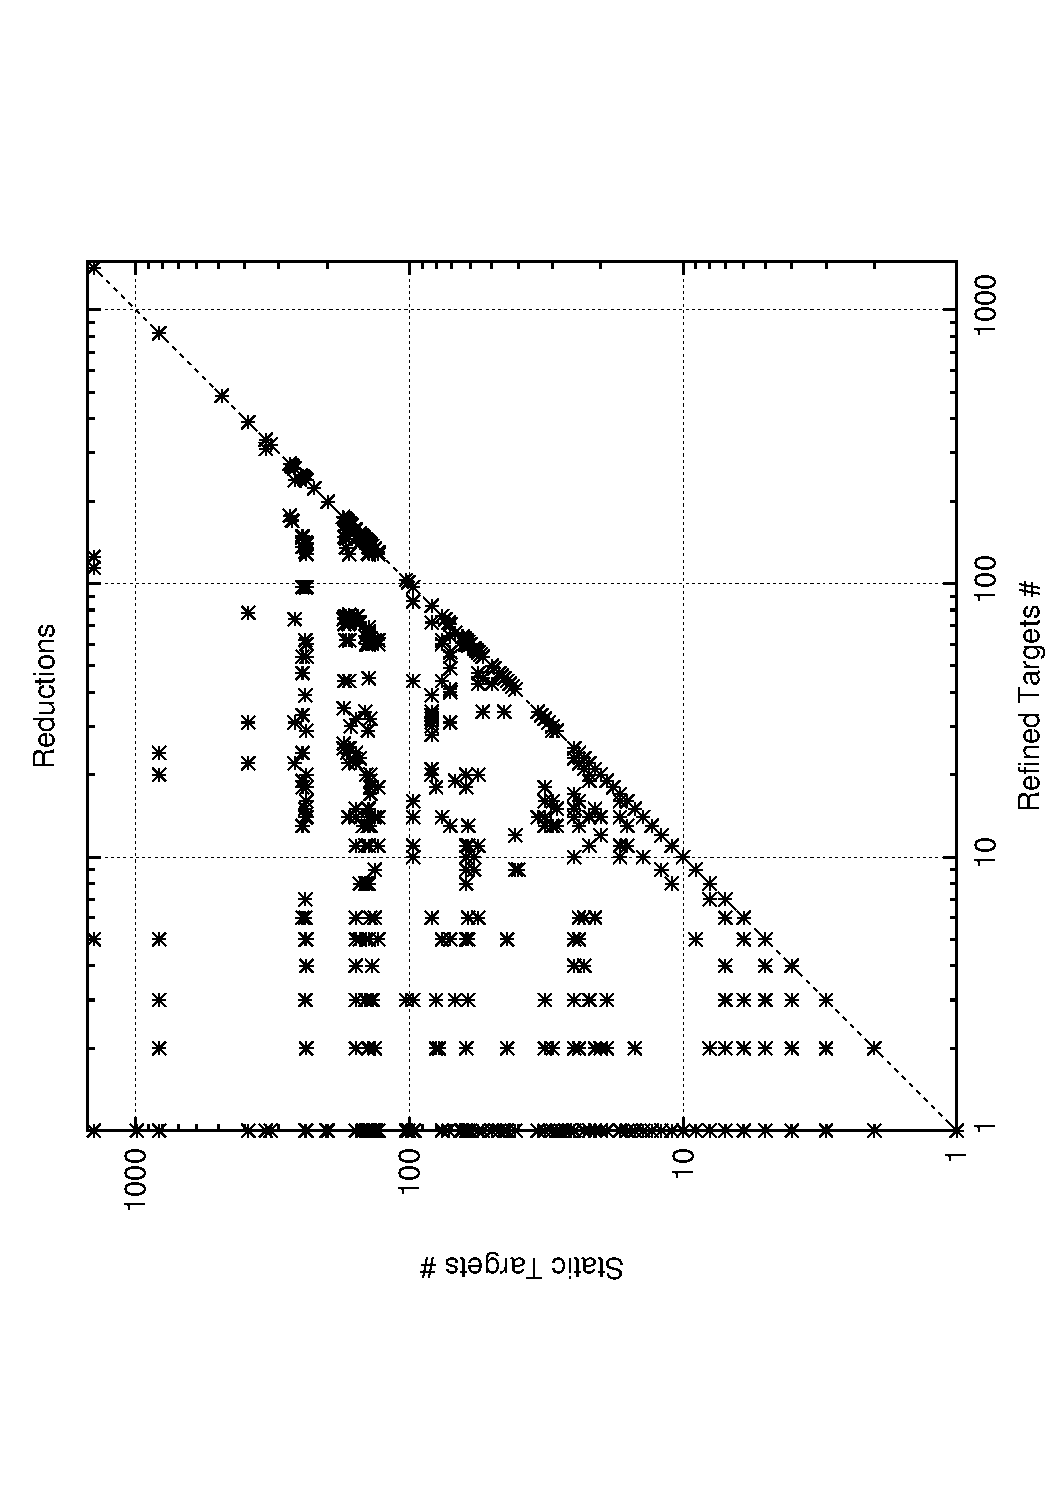
\includegraphics[scale=0.6]{images/scatter}
    \end{center}
    \caption{Improvements due to Type Analysis. Each point represent targets
    computed for one method call. Points on the diagonal represent calls
    without improvements. Points on the Y axis represent calls where the
    analysis reduced the number of targets to a single method.}
    \label{fig:scatter}
\end{figure}

\section{Pointer and Effect Analysis}
\subsection{Overview}
The problem of analyzing pointers is closely related to the field of effects
analysis. Indeed, establishing the relationships between pointers require
understanding how and to what values fields are written to. Because of this
strong inter-dependence, it is profitable to perform both analyses simultaneously.

Our analysis builds summaries of methods, both in terms of their effects and in
terms of the shape of the heap.

\subsection{Flexible Summaries}
Previously, the analysis computed one single, graph-based representation of the
effects of a function. This requires that all method calls have been resolved
and their effects have been merged in. This approach failed to precisely handle
code that highly depends on dynamic dispatch, such as code relying on higher
order functions (HOF).

The main problem when analyzing higher-order functions is that the effect of a
procedure taking a function as argument is directly dependant the actual
argument value. This would require a strongly context-sensitive analysis, which
is usually not compatible with a modular and compositional analysis. It is our
belief that the only way to handle such cases presicely and modularly is to
allow for unresolved method calls to be part of our effect summaries.

Given our previous summaries it is not clear how to include unresolved method
calls in a sound fashion. Instead, we decided to start from CFGs and replace
statements that are precise enough with partial effect "statements". We thus
obtain modified CFGs as effect summaries, granting us a lot of flexibility in
terms of precision: imprecise method calls remain as-is, and their surroundings
that are precise enough can get summarized and grouped into partial effects.

It is important to understand that while we modified our summaries, the
abstract domain and the lattice used in the AI-based analysis remains simple
effect graphs.

\subsubsection{Difficulties of CFG-based Summaries}

The use of CFGs as compositional summaries has a few caveats that needed to be
addressed:

\paragraph{Fix-point Algorithm} When encountering a method call during our
dataflow analysis, we will potentially need to inline a \emph{non-flat} effect
(We say that an effect summary is \emph{flat} if it contains only one single
effect statement, in other words it is fully reduced). This will modify the CFG
being analyzed and the fix-point algorithm needs to take this into account. A
trivial way of handling such modifications is to restart the analysis from
scratch. We however implemented partial restart, which only restarts the
fix-point computation on the corresponding strongly connected component of the
CFG.

\paragraph{Termination Argument} The usual arguments necessary to prove the
termination of the fix-point algorithm are not sufficient in our case. We need
to prove that not only the CFGs are modified in a monotonous fashion, but also
that they themselves reach a fixpoint. In order to make sure that the CFG does
not keep changing, we need to prevent the inlining of recursive or mutualy
recursive functions.


\paragraph{Variable Versionning} Local variables inlined from distinct method
calls need to be disambiguated. We thus had to introduce variable versionning
to separate them appropriately.


\subsection{Context-Sensitivity}
In some cases, the static signature of a method is not precise enough to
compute meaningful and reusable flat effects, for that reason, we decided to
implement some context-sensitivity in our analysis: when the analysis of some
method call requests some effects, it provides the call-site type signature in
the request.

From that, some heuristic decides whether it should reanalyze the function
based on the new call-signature and the effects computed for other signatures.
Currently, the analysis will re-analyze for any new signature, but this could
be refined in the future for better performance.

\section{Future Work}
We can identify multiple ideas for further development:

\subsection{Refined Context-Sensitivity}
Instead of reanalyzing whenever the type signature changes, we could instead
identify arguments that may have a big effect on the precision of the analysis
One possible way to detect such relevant arguments is to see if they are either
involved in imprecise method calls, or passed as relevant arguments to other
methods.

\subsection{Partial Reductions}
Currently, the reduction performed on effects are trivial: if any method call
has not been analyzed, it will not reduce the current CFG. If everything could
be analyzed, it will reduce to a flat effect. We currently do not partially
reduce effects to keep only relevant method calls as precise. Doing so would
improve the performance of the analysis dramatically.

\subsection{Improved Heuristic for Precise v.s. Flat inlining}
Currently, the criteria to inline a method call as a flat effect depends on the
call signature: If all arguments have a single static type, we always inline as
a flat effect. This is however suboptimal for two main reasons:
\begin{enumerate}
    \item We may want to use flat inlining even if not all arguments are not fully
precise, it might be the case if the argument is not relevant for the effect
computation.
    \item The type of the argument being precise is not precise enough, we might
benefit from inlining as a CFG. For instance, if the target method calls a
method on a field of the passed argument.
\end{enumerate}

\end{document}
